\documentclass[a4paper,12pt,french]{article}

\usepackage[TD]{../../Style}

%\renewenvironment{center}{\par \centering }{ \par}
%\renewenvironment{multicols*}[1]{}{}
%\setstretch{1.2}
\renewcommand{\arraystretch}{1.8}
% Début du document
%%%%%%%%%%%%%%%%%%%
\begin{document}

\titre{Problèmes}

\begin{multicols*}{2}
\begin{probleme}
Vrai ou faux? Justifier.

\begin{enumerate}
\item La somme de deux nombres décimaux est un nombre décimal.
\item Pour tout $n \in \N$, $\sqrt n$ est un nombre irrationnel.
\item La somme de deux nombres irrationnels est un nombre irrationnel.
\item Un élève répond au hasard et de manière équiprobable aux cinq questions d'un questionnaire de type \og Vrai ou faux \fg.
\begin{enumerate}
\item La probabilité qu'il ait cinq réponses correctes est égale $\frac 1 {32}$.
\item La probabilité qu'il ait exactement trois réponses correctes est égale $\frac {10} {32}$.
\end{enumerate}
\end{enumerate}
\end{probleme}

\begin{defins}
Etant donnés deux nombres réels $a$ et $b$ positifs, on appelle:
\begin{itemize}
\item Moyenne arithmétique de $a$ et $b$ le nombre: $$m:=\frac{a+b} 2$$
\item Moyenne quadratique de $a$ et $b$ le nombre: $$q:=\sqrt{\frac{a^2+b^2} 2}$$
\item Moyenne géométrique de $a$ et $b$ le nombre: $$g:=\sqrt{ab}$$
\item Si de plus $a$ et $b$ sont strictement positifs, on appelle moyenne harmonique de $a$ et $b$ le nombre: $$h:=\frac 1 2 \left( \frac 1 a + \frac a b \right)$$
\end{itemize}
\end{defins}

\begin{probleme}
Lors d'un premier contrôle, un élève a obtenu la note de 9 sur 20. Un deuxième contrôle est prévu, avec le même coefficient que le premier.

Quelle est la valeur maximale de la moyenne que cet élève 
peut obtenir sur ces deux notes ?
\end{probleme}

\begin{probleme}
Entre octobre 2018 et novembre 2018, le prix baril de pétrole brut de la mer du Nord a connu une baisse de 19\%.
\begin{itemize}
\item Entre novembre 2018 et décembre 2018, il a connu une nouvelle baisse de 12\%.
\item Entre décembre 2018 et janvier 2019, il a connu une hausse de 4\%.
\end{itemize}

\begin{enumerate}
\item Calculer le taux d'évolution mensuel moyen entre octobre 2018 et décembre 2018, puis entre novembre 2018 et janvier 2019.
\item Quel type de moyenne ce problème met-il en jeu ?
\end{enumerate}
\end{probleme}

\begin{probleme}
On dispose de deux plaques métalliques de formes cylindriques, de même épaisseur
$e = 20$cm, mais de rayons différents $R_1 = 30$cm et $R_2 = 50$cm. On décide de fondre
ces deux plaques pour en fabriquer deux autres, de même épaisseur e et de même
rayon $R$.

\begin{enumerate}
\item Calculer $R$.
\item Quel type de moyenne ce problème met-il en jeu ?
\end{enumerate}

\end{probleme}

\begin{probleme}
Un cycliste effectue la montée d'un col à la vitesse constante $v_1 = 20$km/h. Une fois arrivé au col, il redescend par la même route à la vitesse constante $v_2 = 60$km/h.
\begin{enumerate}
\item Calculer sa vitesse moyenne sur l'ensemble du trajet.
\item Quel type de moyenne ce problème met-il en jeu ?
\end{enumerate}
\end{probleme}

\begin{probleme}
Une loi physique, la loi d'Archimède, permet d'affirmer que la balance ci-dessous est en équilibre si $m \times l = m' \times l'$ où $m$ et $m'$ sont les masses posées sur chaque plateau et $l$ et $l'$ sont respectivement les longueurs $OA$ et $OB$ des deux fléaux de la balance.

\begin{center}
\begin{resizetikz}{0.9\linewidth}
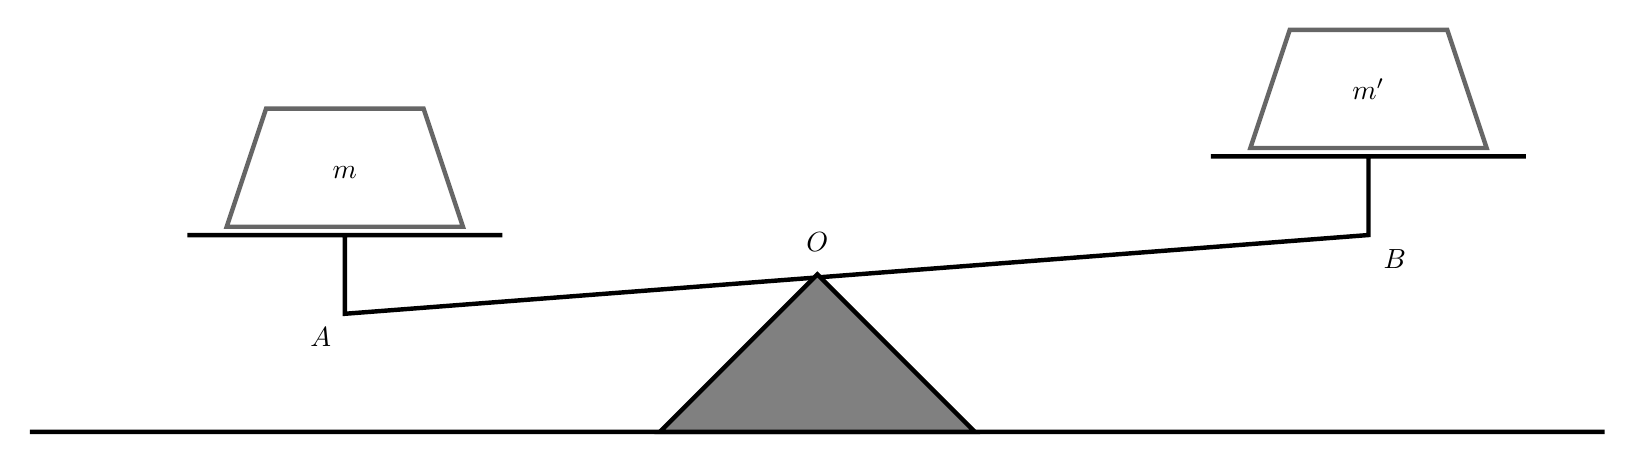
\begin{tikzpicture}
\draw[ultra thick]
(-10,0) -- (10,0)
(-8,2.5) -- (-4,2.5)
(-6,2.5) -- (-6,1.5) node[inner sep=0pt,minimum width=0pt,label=-135:$A$] (A) {} -- (7,2.5) node[inner sep=0pt,label=-45:$B$] (B) {} -- (7,3.5)
(5,3.5) -- (9,3.5);
\draw[ultra thick,fill=black!50] (-2,0) -- (0,2) node[label=90:$O$] (O) {} -- (2,0) -- cycle;

\draw[ultra thick,yshift=3pt,draw=black!60] (-7.5,2.5) -- (-4.5,2.5) -- (-5,4) -- (-7,4) -- cycle;
\node at (-6,3.3) {\strut $m$};

\draw[ultra thick,yshift=3pt,draw=black!60] (8.5,3.5) -- (5.5,3.5) -- (6,5) -- (8,5) -- cycle;
\node[baseline=0pt] at (7,4.3) {\strut $m'$};
\end{tikzpicture}
\end{resizetikz}
\end{center}

On souhaite déterminer la masse $x$ d'un objet. On ne connaît pas les longueurs $l$ et $l'$ et on ne peut pas les mesurer. On dispose en revanche de diverses masses marquées. On réalise une première pesée, où l'équilibre est réalisé pour une masse $m$, conformément au schéma ci-dessous.

\begin{center}
\begin{resizetikz}{0.9\linewidth}
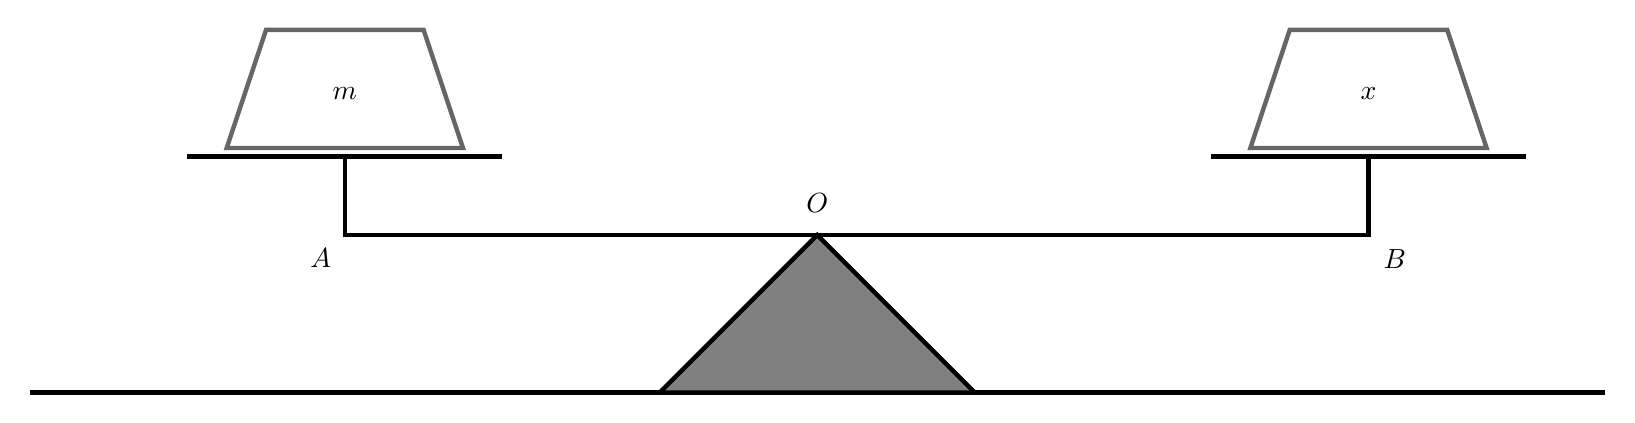
\begin{tikzpicture}
\draw[ultra thick]
(-10,0) -- (10,0)
(-8,3) -- (-4,3)
(-6,3) -- (-6,2) node[inner sep=0pt,minimum width=0pt,label=-135:$A$] (A) {} -- (7,2) node[inner sep=0pt,label=-45:$B$] (B) {} -- (7,3)
(5,3) -- (9,3);
\draw[ultra thick,fill=black!50] (-2,0) -- (0,2) node[label=90:$O$] (O) {} -- (2,0) -- cycle;

\draw[ultra thick,yshift=3pt,draw=black!60] (-7.5,3) -- (-4.5,3) -- (-5,4.5) -- (-7,4.5) -- cycle;
\node at (-6,3.8) {\strut $m$};

\draw[ultra thick,yshift=3pt,draw=black!60] (8.5,3) -- (5.5,3) -- (6,4.5) -- (8,4.5) -- cycle;
\node[baseline=0pt] at (7,3.8) {\strut $x$};
\end{tikzpicture}
\end{resizetikz}
\end{center}

On réalise une seconde pesée, où l'équilibre est réalisé pour une masse $m'$, conformément au schéma ci-dessous.

\begin{center}
\begin{resizetikz}{0.9\linewidth}
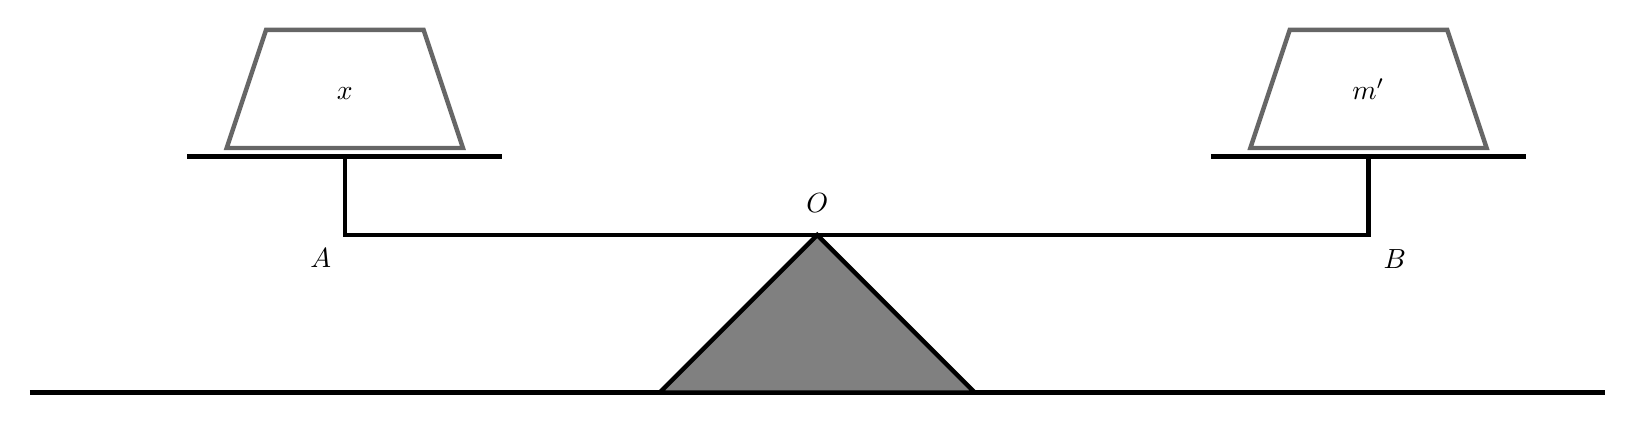
\begin{tikzpicture}
\draw[ultra thick]
(-10,0) -- (10,0)
(-8,3) -- (-4,3)
(-6,3) -- (-6,2) node[inner sep=0pt,minimum width=0pt,label=-135:$A$] (A) {} -- (7,2) node[inner sep=0pt,label=-45:$B$] (B) {} -- (7,3)
(5,3) -- (9,3);
\draw[ultra thick,fill=black!50] (-2,0) -- (0,2) node[label=90:$O$] (O) {} -- (2,0) -- cycle;

\draw[ultra thick,yshift=3pt,draw=black!60] (-7.5,3) -- (-4.5,3) -- (-5,4.5) -- (-7,4.5) -- cycle;
\node at (-6,3.8) {\strut $x$};

\draw[ultra thick,yshift=3pt,draw=black!60] (8.5,3) -- (5.5,3) -- (6,4.5) -- (8,4.5) -- cycle;
\node[baseline=0pt] at (7,3.8) {\strut $m'$};
\end{tikzpicture}
\end{resizetikz}
\end{center}

\begin{enumerate}
\item Exprimer $x$ en fonction de $m$ et $m'$.
\item Quel type de moyenne ce problème met-il en jeu?
\end{enumerate}
\end{probleme}

\begin{probleme}
Un bricoleur désire faire des travaux dans une pièce schématisée ci-dessous (la figure n'est pas à l'échelle).

\begin{center}
\begin{resizetikz}{\linewidth}
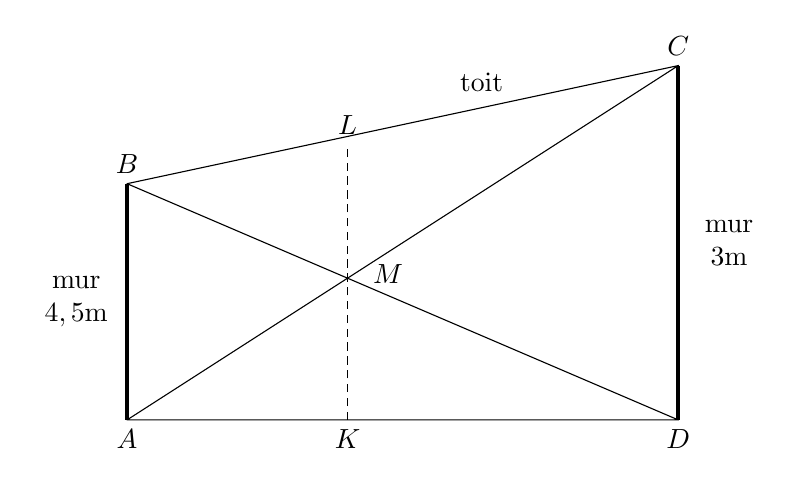
\begin{tikzpicture} % Fait à l'arrache, librairie intersections à utiliser
\coordinate[label=-90:$A$] (A) at (0,0);
\coordinate[label=90:$B$] (B) at (0,3);
\coordinate[label=90:$C$] (C) at (7,4.5);
\coordinate[label=-90:$D$] (D) at (7,0);

\draw (A) -- (B) -- (C) -- (D) -- cycle (B) -- (D) (A) -- (C) (B) -- (C) node[pos=0.7,above left] {toit};
\draw[ultra thick] (A) -- (B) node[pos=0.5,left,text width=1cm,text centered] {mur $4,5$m} (C) -- (D) node[pos=0.5,right,text width=1cm,text centered] {mur $3$m};

\coordinate[label=-90:$K$] (K) at (2.8,0);
\coordinate[label=90:$L$] (L) at (2.8,3.5);
\coordinate[label=0:$M$] (M) at (3,1.85);

\draw[densely dashed] (K) -- (L);
\end{tikzpicture}
\end{resizetikz}
\end{center}

Les segments $[AC]$ et $[BD]$ représentent deux échelles posées l'une contre l'autre qui se croisent en $M$. On pose $a=AB = 3$m et $b=CD=4,5$m. Le bricoleur mesure $1,75$m et se pose plusieurs questions:
\begin{itemize}
\item Peut-il passer sous les échelles sans avoir à se baisser?
\item S'il monte s'installer en $M$, pourra-t-il rester debout sans atteindre le toit ou devra-t-il s'accroupir?
\item Quelle serait la hauteur d'une cloison joignant les points $K$ et $L$?
\end{itemize}
\begin{enumerate}
\item En appliquant le théorème de Thalès à des configuration que l'on précisera, démontrer que:
$$\begin{aligned} \frac b {KM} = 1 + \frac{MC}{MA} \\ \frac a {ML} = 1 + \frac {MA} {MC} \\ \frac {MB} {MD} = \frac {MA} {MC} = \frac a b \end{aligned}$$
\item Répondre à chacune des questions que se pose le bricoleur.
\item Exprimer $KL$ sous la forme de l'une des moyennes de $a$ et $b$.
\end{enumerate}
\end{probleme}

\begin{probleme}
Dans un triangle $AMB$ rectangle en $M$, on note $H$ le pied de la hauteur issue de $M$. On désigne par $a$ la longueur du segment $[HA]$ et $b$ celle du segment $[HB]$.
\begin{enumerate}
\item Démontrer que les triangles $AHM$ et $MHB$ sont semblables et en déduire la longueur $MH$ en fonction de $a$ et $b$.
\item Quel type de moyenne ce problème met-il en jeu?
\end{enumerate}
\end{probleme}

\begin{probleme}
Construire une figure d'après la description suivante: Soit $[AB]$ un segment de milieu $O$. Tracer $\Gamma$ un demi-cercle de diamètre $[AB]$. On considère un point $H$ du segment $[OA]$, distinct de $O$ et de $A$. On pose $ÂH=a$ et $HB=b$. On complètera la figure au fur et à mesure.
\begin{enumerate}
\item Exprimer $OM$ en fonction de $a$ et $b$. La longueur $OM$ représente une certaine moyenne des nombres $a$ et $b$. Préciser laquelle.
\item Montrer que $MH^2=ab$. La longueur $MH$ représente une certaine moyenne des nombres $a$ et $b$. Préciser laquelle.
\item Soit $\Gamma'$ le demi-cercle de centre $O$ passant par $H$ qui coupe le segment $[OM]$. La perpendiculaire en $O$ à la droite $(OM)$ coupe $\Gamma'$ en $G$. Exprimer $OG$ en fonction de $a$ et $b$.
\item En déduire une expression de $MG$ en fonction de $a$ et $b$. La longueur $MG$ représente une certaine moyenne des nombres $a$ et $b$. Préciser laquelle.
\item On considère le point $N$ du segment $[OM]$ tel que $MN = MH$. La parallèle à la droite $(AB)$ passant par $N$ coupe le segment $[MH]$ en $K$. Exprimer $MK$ en fonction de $a$ et $b$. La longueur $MK$ représente une certaine moyenne des nombres $a$ et $b$. Préciser laquelle.
\end{enumerate}
\end{probleme}
\end{multicols*}
\end{document}
